\documentclass[12pt]{report} 
\usepackage{hyperref}
\hypersetup{colorlinks=true,linkcolor=blue}
\usepackage{theorem,graphicx}
\usepackage{listings,alltt}
\bibliographystyle{plain}


\lstset{ %configuring the display of scilab codes
             tabsize=4,
             language=scilab,
             basicstyle=\ttfamily,
             aboveskip={1\baselineskip},
             showstringspaces=false,
             breaklines=true,
             showspaces=false,
             numbers=left,
             numberstyle=\small,
             stringstyle=\normalfont,
             keywordstyle=\color{red},
             emph={clc, all, gca},
             emphstyle=\color{red},
             commentstyle=\color{blue}\normalfont}

 
% code environment
{\theorembodyfont{\rmfamily} \newtheorem{codemass}{Scilab code}[chapter]}
\newenvironment{code}%
{\begin{codemass}}{\hrule \end{codemass}}

{\theorembodyfont{\rmfamily} \newtheorem{accmass}{Acc}[chapter]}
\newenvironment{acc-code}%
{\begin{accmass}}{\end{accmass}}


% create listing for code

\newcommand\tcaption[1]
     {\addcontentsline{cod}{section}{\protect\numberline {\thecodemass}#1}}
\makeatletter \newcommand\listofcode
     {\chapter*{List of Scilab Codes\markboth%
                        {\bf List of Scilab Codes}{}}%
\renewcommand*\l@section{\@dottedtocline{1}{1.5em}{5em}}%
\addcontentsline{toc}{chapter}{\protect\numberline{List of Scilab Codes}}
\@starttoc{cod}}
\newcommand\l@matlab[3]
     {#1 \par\noindent#2, #3 \par}
\renewcommand\@pnumwidth{2.1em}
%\makeatother

\makeatletter
\def\curlable#1{\def\thecodemass{#1}\def\@currentlabel{#1}}
\makeatother

\newcommand{\coderef}[1]{Exa~\ref{#1}}
\newcommand{\figref}[1]{Fig.~\ref{#1}}

\title{Scilab Textbook Companion for \\ELECTRONIC DEVICES\\by THOMAS L FLOYD\footnote{Funded by a grant from the National Mission on Education through ICT, http://spoken-tutorial.org/NMEICT-Intro. This Textbook Companion and Scilab codes written in it can be downloaded from the "Textbook Companion Project" section at the website http://scilab.in}}
\author{ Created by \\PRAVEENA DEVAGUPTA\\B.TECH\\Electronics Engineering,NIT Karnataka, Surathkal\\ College Teacher\\Dr.Laxminidhi T, NIT Surathkal\\Cross-Checked by \\\\}
\date{\today}
\begin{document}
\maketitle

\chapter*{Book Description}
\begin{description}
\item [Title:] ELECTRONIC DEVICES
\item [Author:] THOMAS L FLOYD
\item [Publisher:] Dorling Kindersley Pvt. Ltd
\item [Edition:] 7
\item [Year:] 2009
\item [ISBN:] 81-7758-643-5
\end{description}

\newpage
\vspace*{3cm}
Scilab numbering policy used in this document and the relation to the above book.
\begin{description}
\item[Exa] Example (Solved example)
\item[Eqn] Equation (Particular equation of the above book)
\item[AP] Appendix to Example(Scilab Code that is an Appednix to a particular Example of the above book)
\end{description}
For example, Exa~3.51 means solved example 3.51 of this book. Sec~2.3 means a scilab code whose theory is explained in Section 2.3 of the book.

\tableofcontents
\listofcode
\listoffigures

\chapter{semiconductor basics}

\vspace*{10mm}
\curlable{Exa~1.1}
\begin{code}
\tcaption{Different diode models}{Different diode models}
\lstinputlisting{../61/CH1/EX1.1/ex1_1.sce}
\end{code}

\chapter{diode applications}

\vspace*{10mm}
\curlable{Exa~2.1}
\begin{code}
\tcaption{Average value half wave rectifier}{Average value half wave rectifier}
\lstinputlisting{../61/CH2/EX2.1/ex2_1.sce}
\end{code}

\vspace*{10mm}
\curlable{Fig~2.2.a}
\begin{figure}
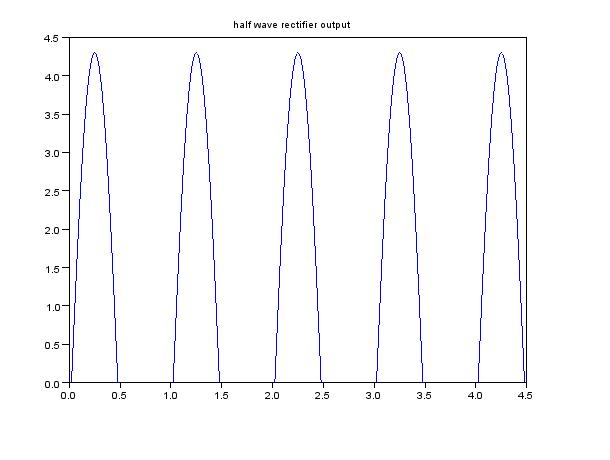
\includegraphics[width=6in]{../61/CH2/EX2.2.a/ex2_2a.jpg}
\caption{half wave rectifier}
\end{figure}

\vspace*{10mm}
\curlable{Exa~2.2.a}
\begin{code}
\tcaption{half wave rectifier}{half wave rectifier}
\lstinputlisting{../61/CH2/EX2.2.a/ex2_2a.sce}
\end{code}

\vspace*{10mm}
\vspace*{10mm}
\curlable{Exa~2.2.b}
\begin{code}
\tcaption{half wave rectifier}{half wave rectifier}
\lstinputlisting{../61/CH2/EX2.2.b/ex2_2b.sce}
\end{code}

\vspace*{10mm}
\curlable{Exa~2.3}
\begin{code}
\tcaption{Rectifier peak value}{Rectifier peak value}
\lstinputlisting{../61/CH2/EX2.3/ex2_3.sce}
\end{code}

\vspace*{10mm}
\curlable{Exa~2.4}
\begin{code}
\tcaption{Average value full wave rectifier}{Average value full wave rectifier}
\lstinputlisting{../61/CH2/EX2.4/ex2_4.sce}
\end{code}

\vspace*{10mm}
\curlable{Fig~2.5}
\begin{figure}
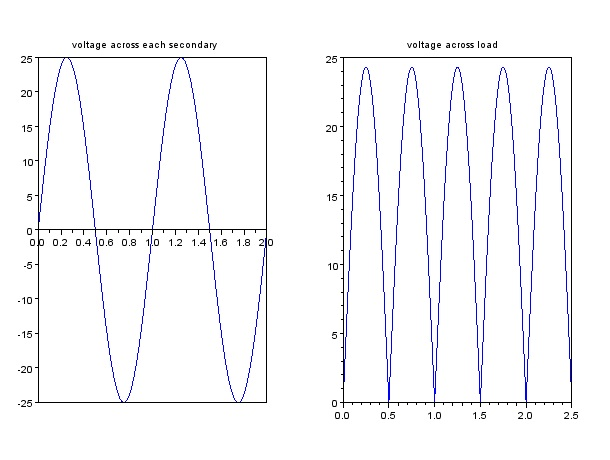
\includegraphics[width=6in]{../61/CH2/EX2.5/ex2_5.jpg}
\caption{PIV full wave}
\end{figure}

\vspace*{10mm}
\curlable{Exa~2.5}
\begin{code}
\tcaption{PIV full wave}{PIV full wave}
\lstinputlisting{../61/CH2/EX2.5/ex2_5.sce}
\end{code}

\vspace*{10mm}
\curlable{Exa~2.6}
\begin{code}
\tcaption{Bridge Rectifier}{Bridge Rectifier}
\lstinputlisting{../61/CH2/EX2.6/ex2_6.sce}
\end{code}

\vspace*{10mm}
\curlable{Exa~2.7}
\begin{code}
\tcaption{Ripple Bridge rectifier}{Ripple Bridge rectifier}
\lstinputlisting{../61/CH2/EX2.7/ex2_7.sce}
\end{code}

\vspace*{10mm}
\curlable{Exa~2.8}
\begin{code}
\tcaption{Voltage Regulator}{Voltage Regulator}
\lstinputlisting{../61/CH2/EX2.8/ex2_8.sce}
\end{code}

\vspace*{10mm}
\curlable{Exa~2.9}
\begin{code}
\tcaption{Load regulation percentage}{Load regulation percentage}
\lstinputlisting{../61/CH2/EX2.9/ex2_9.sce}
\end{code}

\vspace*{10mm}
\curlable{Fig~2.10}
\begin{figure}
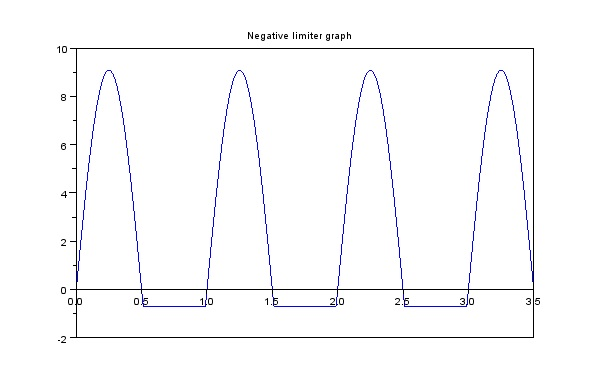
\includegraphics[width=6in]{../61/CH2/EX2.10/ex2_10.jpg}
\caption{Negative diode limiter}
\end{figure}

\vspace*{10mm}
\curlable{Exa~2.10}
\begin{code}
\tcaption{Negative diode limiter}{Negative diode limiter}
\lstinputlisting{../61/CH2/EX2.10/ex2_10.sce}
\end{code}

\vspace*{10mm}
\curlable{Fig~2.11}
\begin{figure}
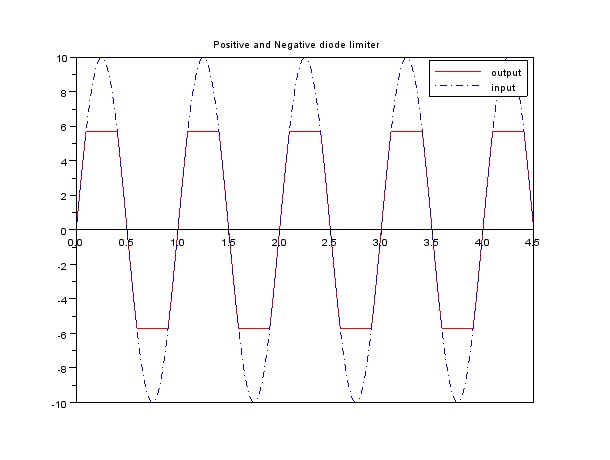
\includegraphics[width=6in]{../61/CH2/EX2.11/ex2_11.jpg}
\caption{Posiive Negative Limiter}
\end{figure}

\vspace*{10mm}
\curlable{Exa~2.11}
\begin{code}
\tcaption{Posiive Negative Limiter}{Posiive Negative Limiter}
\lstinputlisting{../61/CH2/EX2.11/ex2_11.sce}
\end{code}

\vspace*{10mm}
\curlable{Fig~2.12}
\begin{figure}
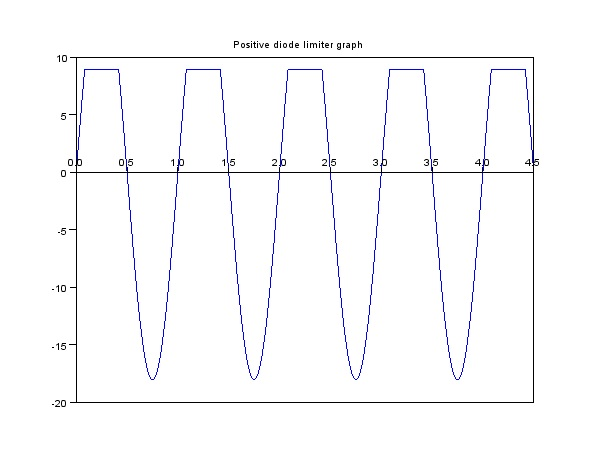
\includegraphics[width=6in]{../61/CH2/EX2.12/ex2_12.jpg}
\caption{Positive diode limiter}
\end{figure}

\vspace*{10mm}
\curlable{Exa~2.12}
\begin{code}
\tcaption{Positive diode limiter}{Positive diode limiter}
\lstinputlisting{../61/CH2/EX2.12/ex2_12.sce}
\end{code}

\vspace*{10mm}
\curlable{Fig~2.13}
\begin{figure}
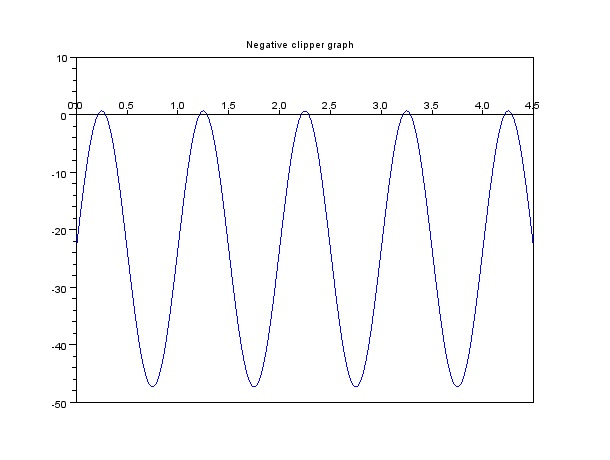
\includegraphics[width=6in]{../61/CH2/EX2.13/ex2_13.jpg}
\caption{Negative Clamper}
\end{figure}

\vspace*{10mm}
\curlable{Exa~2.13}
\begin{code}
\tcaption{Negative Clamper}{Negative Clamper}
\lstinputlisting{../61/CH2/EX2.13/ex2_13.sce}
\end{code}

\chapter{Special purpose diodes}

\vspace*{10mm}
\curlable{Exa~3.1}
\begin{code}
\tcaption{Zener impedance}{Zener impedance}
\lstinputlisting{../61/CH3/EX3.1/ex3_1.sce}
\end{code}

\vspace*{10mm}
\curlable{Exa~3.2}
\begin{code}
\tcaption{Zener Voltage}{Zener Voltage}
\lstinputlisting{../61/CH3/EX3.2/ex3_2.sce}
\end{code}

\vspace*{10mm}
\curlable{Exa~3.3}
\begin{code}
\tcaption{Temperature coefficient}{Temperature coefficient}
\lstinputlisting{../61/CH3/EX3.3/ex3_3.sce}
\end{code}

\vspace*{10mm}
\curlable{Exa~3.4}
\begin{code}
\tcaption{Zener power dissipation}{Zener power dissipation}
\lstinputlisting{../61/CH3/EX3.4/ex3_4.sce}
\end{code}

\vspace*{10mm}
\curlable{Exa~3.5}
\begin{code}
\tcaption{Zener voltage regulator}{Zener voltage regulator}
\lstinputlisting{../61/CH3/EX3.5/ex3_5.sce}
\end{code}

\vspace*{10mm}
\curlable{Exa~3.6}
\begin{code}
\tcaption{Regulation Variable load}{Regulation Variable load}
\lstinputlisting{../61/CH3/EX3.6/ex3_6.sce}
\end{code}

\vspace*{10mm}
\curlable{Exa~3.7}
\begin{code}
\tcaption{Zener regulation}{Zener regulation}
\lstinputlisting{../61/CH3/EX3.7/ex3_7.sce}
\end{code}

\vspace*{10mm}
\curlable{Fig~3.8}
\begin{figure}
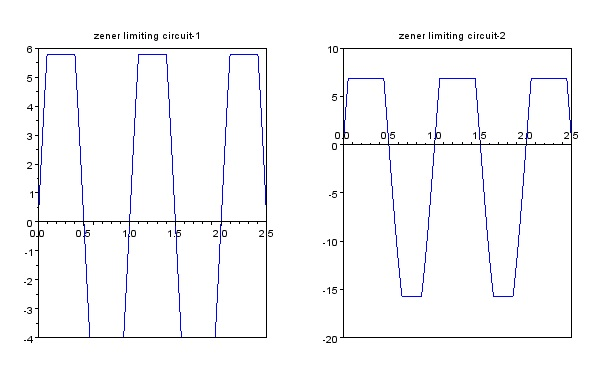
\includegraphics[width=6in]{../61/CH3/EX3.8/ex3_8.jpg}
\caption{Zener limiting}
\end{figure}

\vspace*{10mm}
\curlable{Exa~3.8}
\begin{code}
\tcaption{Zener limiting}{Zener limiting}
\lstinputlisting{../61/CH3/EX3.8/ex3_8.sce}
\end{code}

\chapter{Bipolar Junction Transistors}

\vspace*{10mm}
\curlable{Exa~4.1}
\begin{code}
\tcaption{DC beta}{DC beta}
\lstinputlisting{../61/CH4/EX4.1/ex4_1.sce}
\end{code}

\vspace*{10mm}
\curlable{Exa~4.2}
\begin{code}
\tcaption{Current Voltage Analysis}{Current Voltage Analysis}
\lstinputlisting{../61/CH4/EX4.2/ex4_2.sce}
\end{code}

\vspace*{10mm}
\curlable{Exa~4.3}
\begin{code}
\tcaption{Collector characteristic curve}{Collector characteristic curve}
\lstinputlisting{../61/CH4/EX4.3/ex4_3.sce}
\end{code}

\vspace*{10mm}
\curlable{Exa~4.4}
\begin{code}
\tcaption{DC loadline}{DC loadline}
\lstinputlisting{../61/CH4/EX4.4/ex4_4.sce}
\end{code}

\vspace*{10mm}
\curlable{Exa~4.5}
\begin{code}
\tcaption{Transistor rating}{Transistor rating}
\lstinputlisting{../61/CH4/EX4.5/ex4_5.sce}
\end{code}

\vspace*{10mm}
\curlable{Exa~4.6}
\begin{code}
\tcaption{Maximum Transistor Rating}{Maximum Transistor Rating}
\lstinputlisting{../61/CH4/EX4.6/ex4_6.sce}
\end{code}

\vspace*{10mm}
\curlable{Exa~4.7}
\begin{code}
\tcaption{Derating Power maximum}{Derating Power maximum}
\lstinputlisting{../61/CH4/EX4.7/ex4_7.sce}
\end{code}

\vspace*{10mm}
\curlable{Exa~4.8}
\begin{code}
\tcaption{Transistor amplification}{Transistor amplification}
\lstinputlisting{../61/CH4/EX4.8/ex4_8.sce}
\end{code}

\vspace*{10mm}
\curlable{Exa~4.9}
\begin{code}
\tcaption{Collector in saturation}{Collector in saturation}
\lstinputlisting{../61/CH4/EX4.9/ex4_9.sce}
\end{code}

\chapter{Transistor Bias Circuits}

\vspace*{10mm}
\curlable{Exa~5.1}
\begin{code}
\tcaption{DC bias}{DC bias}
\lstinputlisting{../61/CH5/EX5.1/ex5_1.sce}
\end{code}

\vspace*{10mm}
\curlable{Exa~5.2}
\begin{code}
\tcaption{Input resistance}{Input resistance}
\lstinputlisting{../61/CH5/EX5.2/ex5_2.sce}
\end{code}

\vspace*{10mm}
\curlable{Exa~5.3}
\begin{code}
\tcaption{Voltage divider bias}{Voltage divider bias}
\lstinputlisting{../61/CH5/EX5.3/ex5_3.sce}
\end{code}

\vspace*{10mm}
\curlable{Exa~5.4}
\begin{code}
\tcaption{Voltage bias PNP}{Voltage bias PNP}
\lstinputlisting{../61/CH5/EX5.4/ex5_4.sce}
\end{code}

\vspace*{10mm}
\curlable{Exa~5.5}
\begin{code}
\tcaption{PNP Transistor}{PNP Transistor}
\lstinputlisting{../61/CH5/EX5.5/ex5_5.sce}
\end{code}

\vspace*{10mm}
\curlable{Exa~5.6}
\begin{code}
\tcaption{Qpoint base bias}{Qpoint base bias}
\lstinputlisting{../61/CH5/EX5.6/ex5_6.sce}
\end{code}

\vspace*{10mm}
\curlable{Exa~5.7}
\begin{code}
\tcaption{Emitter bias}{Emitter bias}
\lstinputlisting{../61/CH5/EX5.7/ex5_7.sce}
\end{code}

\vspace*{10mm}
\curlable{Exa~5.8}
\begin{code}
\tcaption{Q point}{Q point}
\lstinputlisting{../61/CH5/EX5.8/ex5_8.sce}
\end{code}

\chapter{BJT Amplifiers}

\vspace*{10mm}
\curlable{Exa~6.1}
\begin{code}
\tcaption{Linear amplifier}{Linear amplifier}
\lstinputlisting{../61/CH6/EX6.1/ex6_1.sce}
\end{code}

\vspace*{10mm}
\curlable{Exa~6.2}
\begin{code}
\tcaption{AC Emitter resistance}{AC Emitter resistance}
\lstinputlisting{../61/CH6/EX6.2/ex6_2.sce}
\end{code}

\vspace*{10mm}
\curlable{Exa~6.3}
\begin{code}
\tcaption{Base voltage}{Base voltage}
\lstinputlisting{../61/CH6/EX6.3/ex6_3.sce}
\end{code}

\vspace*{10mm}
\curlable{Exa~6.4}
\begin{code}
\tcaption{Emitter bypass capacitor}{Emitter bypass capacitor}
\lstinputlisting{../61/CH6/EX6.4/ex6_4.sce}
\end{code}

\vspace*{10mm}
\curlable{Exa~6.5}
\begin{code}
\tcaption{Effect bypass capacitor}{Effect bypass capacitor}
\lstinputlisting{../61/CH6/EX6.5/ex6_5.sce}
\end{code}

\vspace*{10mm}
\curlable{Exa~6.6}
\begin{code}
\tcaption{Gain with load}{Gain with load}
\lstinputlisting{../61/CH6/EX6.6/ex6_6.sce}
\end{code}

\vspace*{10mm}
\curlable{Exa~6.7}
\begin{code}
\tcaption{Gain swamped amplifier}{Gain swamped amplifier}
\lstinputlisting{../61/CH6/EX6.7/ex6_7.sce}
\end{code}

\vspace*{10mm}
\curlable{Fig~6.8}
\begin{figure}
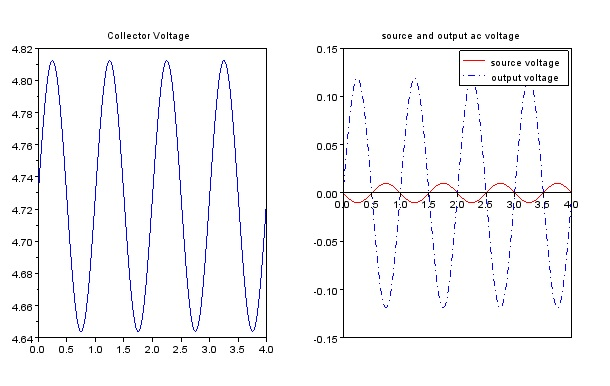
\includegraphics[width=6in]{../61/CH6/EX6.8/ex6_8.jpg}
\caption{Common emitter amplifier}
\end{figure}

\vspace*{10mm}
\curlable{Exa~6.8}
\begin{code}
\tcaption{Common emitter amplifier}{Common emitter amplifier}
\lstinputlisting{../61/CH6/EX6.8/ex6_8.sce}
\end{code}

\vspace*{10mm}
\curlable{Exa~6.9}
\begin{code}
\tcaption{Current gain}{Current gain}
\lstinputlisting{../61/CH6/EX6.9/ex6_9.sce}
\end{code}

\vspace*{10mm}
\curlable{Exa~6.10}
\begin{code}
\tcaption{Darlington emitter follower}{Darlington emitter follower}
\lstinputlisting{../61/CH6/EX6.10/ex6_10.sce}
\end{code}

\vspace*{10mm}
\curlable{Exa~6.11}
\begin{code}
\tcaption{Common base amplifier}{Common base amplifier}
\lstinputlisting{../61/CH6/EX6.11/ex6_11.sce}
\end{code}

\vspace*{10mm}
\curlable{Exa~6.12}
\begin{code}
\tcaption{Voltage gain decibel}{Voltage gain decibel}
\lstinputlisting{../61/CH6/EX6.12/ex6_12.sce}
\end{code}

\chapter{Field Effect Transistors}

\vspace*{10mm}
\curlable{Exa~7.1}
\begin{code}
\tcaption{cutoff FET}{cutoff FET}
\lstinputlisting{../61/CH7/EX7.1/ex7_1.sce}
\end{code}

\vspace*{10mm}
\curlable{Exa~7.2}
\begin{code}
\tcaption{Drain current}{Drain current}
\lstinputlisting{../61/CH7/EX7.2/ex7_2.sce}
\end{code}

check Appendix \ref{AP:4} for dependency: {\begin{alltt} \hspace{2mm} value_of_I_D.sci \end{alltt}}

\vspace*{10mm}
\curlable{Exa~7.3}
\begin{code}
\tcaption{JFET current voltage}{JFET current voltage}
\lstinputlisting{../61/CH7/EX7.3/ex7_3.sce}
\end{code}

check Appendix \ref{AP:4} for dependency: {\begin{alltt} \hspace{2mm} value_of_I_D.sci \end{alltt}}

\vspace*{10mm}
\curlable{Exa~7.4}
\begin{code}
\tcaption{JFET transconductance}{JFET transconductance}
\lstinputlisting{../61/CH7/EX7.4/ex7_4.sce}
\end{code}

\vspace*{10mm}
\curlable{Exa~7.5}
\begin{code}
\tcaption{JFET input resistance}{JFET input resistance}
\lstinputlisting{../61/CH7/EX7.5/ex7_5.sce}
\end{code}

\vspace*{10mm}
\curlable{Exa~7.6}
\begin{code}
\tcaption{Self bias}{Self bias}
\lstinputlisting{../61/CH7/EX7.6/ex7_6.sce}
\end{code}

\vspace*{10mm}
\curlable{Exa~7.7}
\begin{code}
\tcaption{Q point JFET}{Q point JFET}
\lstinputlisting{../61/CH7/EX7.7/ex7_7.sce}
\end{code}

check Appendix \ref{AP:4} for dependency: {\begin{alltt} \hspace{2mm} value_of_I_D.sci \end{alltt}}

\vspace*{10mm}
\curlable{Exa~7.8}
\begin{code}
\tcaption{Self bias Q point}{Self bias Q point}
\lstinputlisting{../61/CH7/EX7.8/ex7_8.sce}
\end{code}

\vspace*{10mm}
\curlable{Exa~7.9}
\begin{code}
\tcaption{Midpoint bias}{Midpoint bias}
\lstinputlisting{../61/CH7/EX7.9/ex7_9.sce}
\end{code}

\vspace*{10mm}
\curlable{Exa~7.10}
\begin{code}
\tcaption{Graphical analysis}{Graphical analysis}
\lstinputlisting{../61/CH7/EX7.10/ex7_10.sce}
\end{code}

\vspace*{10mm}
\curlable{Exa~7.11}
\begin{code}
\tcaption{Voltage Divider bias}{Voltage Divider bias}
\lstinputlisting{../61/CH7/EX7.11/ex7_11.sce}
\end{code}

\vspace*{10mm}
\curlable{Exa~7.12}
\begin{code}
\tcaption{Graph voltage divider}{Graph voltage divider}
\lstinputlisting{../61/CH7/EX7.12/ex7_12.sce}
\end{code}

check Appendix \ref{AP:4} for dependency: {\begin{alltt} \hspace{2mm} value_of_I_D.sci \end{alltt}}

\vspace*{10mm}
\curlable{Exa~7.13}
\begin{code}
\tcaption{DMOSFET}{DMOSFET}
\lstinputlisting{../61/CH7/EX7.13/ex7_13.sce}
\end{code}

check Appendix \ref{AP:5} for dependency: {\begin{alltt} \hspace{2mm} value_of_K.sci \end{alltt}}

\vspace*{10mm}
\curlable{Exa~7.14}
\begin{code}
\tcaption{EMOSFET}{EMOSFET}
\lstinputlisting{../61/CH7/EX7.14/ex7_14.sce}
\end{code}

\vspace*{10mm}
\curlable{Exa~7.15}
\begin{code}
\tcaption{DMOSFET bias}{DMOSFET bias}
\lstinputlisting{../61/CH7/EX7.15/ex7_15.sce}
\end{code}

check Appendix \ref{AP:5} for dependency: {\begin{alltt} \hspace{2mm} value_of_K.sci \end{alltt}}

\vspace*{10mm}
\curlable{Exa~7.16}
\begin{code}
\tcaption{EMOSFET bias}{EMOSFET bias}
\lstinputlisting{../61/CH7/EX7.16/ex7_16.sce}
\end{code}

\vspace*{10mm}
\curlable{Exa~7.17}
\begin{code}
\tcaption{EMOSFET drain current}{EMOSFET drain current}
\lstinputlisting{../61/CH7/EX7.17/ex7_17.sce}
\end{code}

\chapter{FET Amplifiers}

\vspace*{10mm}
\curlable{Exa~8.1}
\begin{code}
\tcaption{Voltage gain}{Voltage gain}
\lstinputlisting{../61/CH8/EX8.1/ex8_1.sce}
\end{code}

\vspace*{10mm}
\curlable{Exa~8.2}
\begin{code}
\tcaption{Rds effect}{Rds effect}
\lstinputlisting{../61/CH8/EX8.2/ex8_2.sce}
\end{code}

\vspace*{10mm}
\curlable{Exa~8.3}
\begin{code}
\tcaption{External source resistance}{External source resistance}
\lstinputlisting{../61/CH8/EX8.3/ex8_3.sce}
\end{code}

\vspace*{10mm}
\curlable{Exa~8.4}
\begin{code}
\tcaption{Unloaded amplifier}{Unloaded amplifier}
\lstinputlisting{../61/CH8/EX8.4/ex8_4.sce}
\end{code}

\vspace*{10mm}
\curlable{Exa~8.5}
\begin{code}
\tcaption{AC load effect}{AC load effect}
\lstinputlisting{../61/CH8/EX8.5/ex8_5.sce}
\end{code}

\vspace*{10mm}
\curlable{Exa~8.6}
\begin{code}
\tcaption{Input resistance}{Input resistance}
\lstinputlisting{../61/CH8/EX8.6/ex8_6.sce}
\end{code}

\vspace*{10mm}
\curlable{Exa~8.7}
\begin{code}
\tcaption{DMOSFET amplifier}{DMOSFET amplifier}
\lstinputlisting{../61/CH8/EX8.7/ex8_7.sce}
\end{code}

\vspace*{10mm}
\curlable{Exa~8.8}
\begin{code}
\tcaption{MOSFET Q points}{MOSFET Q points}
\lstinputlisting{../61/CH8/EX8.8/ex8_8.SCE}
\end{code}

check Appendix \ref{AP:5} for dependency: {\begin{alltt} \hspace{2mm} value_of_K.sci \end{alltt}}

\vspace*{10mm}
\curlable{Exa~8.9}
\begin{code}
\tcaption{EMOSFET amplifier}{EMOSFET amplifier}
\lstinputlisting{../61/CH8/EX8.9/ex8_9.sce}
\end{code}

\vspace*{10mm}
\curlable{Exa~8.10}
\begin{code}
\tcaption{Common gate amplifier}{Common gate amplifier}
\lstinputlisting{../61/CH8/EX8.10/ex8_10.sce}
\end{code}

\chapter{Power Amplifiers}

\vspace*{10mm}
\curlable{Exa~9.1}
\begin{code}
\tcaption{classA power amplifier}{classA power amplifier}
\lstinputlisting{../61/CH9/EX9.1/ex9_1.sce}
\end{code}

\vspace*{10mm}
\curlable{Exa~9.2}
\begin{code}
\tcaption{class A efficiency}{class A efficiency}
\lstinputlisting{../61/CH9/EX9.2/ex9_2.sce}
\end{code}

\vspace*{10mm}
\curlable{Exa~9.3}
\begin{code}
\tcaption{class AB pushpull}{class AB pushpull}
\lstinputlisting{../61/CH9/EX9.3/ex9_3.sce}
\end{code}

\vspace*{10mm}
\curlable{Exa~9.4}
\begin{code}
\tcaption{Single supply pushpull}{Single supply pushpull}
\lstinputlisting{../61/CH9/EX9.4/ex9_4.sce}
\end{code}

\vspace*{10mm}
\curlable{Exa~9.5}
\begin{code}
\tcaption{Power of amplifier}{Power of amplifier}
\lstinputlisting{../61/CH9/EX9.5/ex9_5.sce}
\end{code}

\vspace*{10mm}
\curlable{Exa~9.6}
\begin{code}
\tcaption{MOSFET pushpull amplifier}{MOSFET pushpull amplifier}
\lstinputlisting{../61/CH9/EX9.6/ex9_6.sce}
\end{code}

\vspace*{10mm}
\curlable{Exa~9.7}
\begin{code}
\tcaption{class C amplifier}{class C amplifier}
\lstinputlisting{../61/CH9/EX9.7/ex9_7.sce}
\end{code}

\vspace*{10mm}
\curlable{Exa~9.8}
\begin{code}
\tcaption{class C efficiency}{class C efficiency}
\lstinputlisting{../61/CH9/EX9.8/ex9_8.sce}
\end{code}

\chapter{Amplifier Frequency Response}

check Appendix \ref{AP:6} for dependency: {\begin{alltt} \hspace{2mm} gain_in_decibel_power.sci \end{alltt}}

check Appendix \ref{AP:7} for dependency: {\begin{alltt} \hspace{2mm} gain_in_decibel_voltage.sci \end{alltt}}

\vspace*{10mm}
\curlable{Exa~10.1}
\begin{code}
\tcaption{Gain in decibel}{Gain in decibel}
\lstinputlisting{../61/CH10/EX10.1/ex10_1.sce}
\end{code}

\vspace*{10mm}
\curlable{Exa~10.2}
\begin{code}
\tcaption{Critical frequency}{Critical frequency}
\lstinputlisting{../61/CH10/EX10.2/ex10_2.sce}
\end{code}

\vspace*{10mm}
\curlable{Exa~10.3}
\begin{code}
\tcaption{Lower critical frequency}{Lower critical frequency}
\lstinputlisting{../61/CH10/EX10.3/ex10_3.sce}
\end{code}

\vspace*{10mm}
\curlable{Exa~10.4}
\begin{code}
\tcaption{Voltage gains}{Voltage gains}
\lstinputlisting{../61/CH10/EX10.4/ex10_4.sce}
\end{code}

\vspace*{10mm}
\curlable{Exa~10.5}
\begin{code}
\tcaption{Output RC circuit}{Output RC circuit}
\lstinputlisting{../61/CH10/EX10.5/ex10_5.sce}
\end{code}

\vspace*{10mm}
\curlable{Exa~10.6}
\begin{code}
\tcaption{Bypass RC circuit BJT}{Bypass RC circuit BJT}
\lstinputlisting{../61/CH10/EX10.6/ex10_6.sce}
\end{code}

\vspace*{10mm}
\curlable{Exa~10.7}
\begin{code}
\tcaption{input RC circuit FET}{input RC circuit FET}
\lstinputlisting{../61/CH10/EX10.7/ex10_7.sce}
\end{code}

\vspace*{10mm}
\curlable{Exa~10.8}
\begin{code}
\tcaption{Low frequency response FET}{Low frequency response FET}
\lstinputlisting{../61/CH10/EX10.8/ex10_8.sce}
\end{code}

\vspace*{10mm}
\curlable{Exa~10.9}
\begin{code}
\tcaption{Low frequency response BJT}{Low frequency response BJT}
\lstinputlisting{../61/CH10/EX10.9/ex10_9.sce}
\end{code}

\vspace*{10mm}
\curlable{Exa~10.10}
\begin{code}
\tcaption{input RC circuit BJT}{input RC circuit BJT}
\lstinputlisting{../61/CH10/EX10.10/ex10_10.sce}
\end{code}

\vspace*{10mm}
\curlable{Exa~10.11}
\begin{code}
\tcaption{Critical frequency BJT output}{Critical frequency BJT output}
\lstinputlisting{../61/CH10/EX10.11/ex10_11.sce}
\end{code}

\vspace*{10mm}
\curlable{Exa~10.12}
\begin{code}
\tcaption{FET capacitors}{FET capacitors}
\lstinputlisting{../61/CH10/EX10.12/ex10_12.sce}
\end{code}

\vspace*{10mm}
\curlable{Exa~10.13}
\begin{code}
\tcaption{Critical frequency FET input}{Critical frequency FET input}
\lstinputlisting{../61/CH10/EX10.13/ex10_13.sce}
\end{code}

\vspace*{10mm}
\curlable{Exa~10.14}
\begin{code}
\tcaption{Critical frequency FET input}{Critical frequency FET input}
\lstinputlisting{../61/CH10/EX10.14/ex10_14.sce}
\end{code}

\vspace*{10mm}
\curlable{Exa~10.15}
\begin{code}
\tcaption{Bandwidth}{Bandwidth}
\lstinputlisting{../61/CH10/EX10.15/ex10_15.sce}
\end{code}

\vspace*{10mm}
\curlable{Exa~10.16}
\begin{code}
\tcaption{Bandwidth transistor}{Bandwidth transistor}
\lstinputlisting{../61/CH10/EX10.16/ex10_16.sce}
\end{code}

\vspace*{10mm}
\curlable{Exa~10.17}
\begin{code}
\tcaption{Bandwidth 2stage amplifier}{Bandwidth 2stage amplifier}
\lstinputlisting{../61/CH10/EX10.17/ex10_17.sce}
\end{code}

\vspace*{10mm}
\curlable{Exa~10.18}
\begin{code}
\tcaption{Bandwidth 2stage amplifier}{Bandwidth 2stage amplifier}
\lstinputlisting{../61/CH10/EX10.18/ex10_18.sce}
\end{code}

\chapter{Thyristors and Other Devices}

\vspace*{10mm}
\curlable{Exa~11.1}
\begin{code}
\tcaption{Four layer diode}{Four layer diode}
\lstinputlisting{../61/CH11/EX11.1/ex11_1.sce}
\end{code}

\vspace*{10mm}
\curlable{Exa~11.2}
\begin{code}
\tcaption{Anode current}{Anode current}
\lstinputlisting{../61/CH11/EX11.2/ex11_2.sce}
\end{code}

\vspace*{10mm}
\curlable{Exa~11.3}
\begin{code}
\tcaption{Unijunction transistor}{Unijunction transistor}
\lstinputlisting{../61/CH11/EX11.3/ex11_3.sce}
\end{code}

\vspace*{10mm}
\curlable{Exa~11.4}
\begin{code}
\tcaption{turn on off UJT}{turn on off UJT}
\lstinputlisting{../61/CH11/EX11.4/ex11_4.sce}
\end{code}

\vspace*{10mm}
\curlable{Exa~11.5}
\begin{code}
\tcaption{Critical angle}{Critical angle}
\lstinputlisting{../61/CH11/EX11.5/ex11_5.sce}
\end{code}

\chapter{The Operational Amplifier}

\vspace*{10mm}
\curlable{Exa~12.1}
\begin{code}
\tcaption{CMRR opamp}{CMRR opamp}
\lstinputlisting{../61/CH12/EX12.1/ex12_1.sce}
\end{code}

\vspace*{10mm}
\curlable{Exa~12.2}
\begin{code}
\tcaption{Slew rate}{Slew rate}
\lstinputlisting{../61/CH12/EX12.2/ex12_2.sce}
\end{code}

\vspace*{10mm}
\curlable{Exa~12.3}
\begin{code}
\tcaption{Non inverting amplifier}{Non inverting amplifier}
\lstinputlisting{../61/CH12/EX12.3/ex12_3.sce}
\end{code}

\vspace*{10mm}
\curlable{Exa~12.4}
\begin{code}
\tcaption{Inverting amplifier}{Inverting amplifier}
\lstinputlisting{../61/CH12/EX12.4/ex12_4.sce}
\end{code}

\vspace*{10mm}
\curlable{Exa~12.5}
\begin{code}
\tcaption{Impedance noninverting amplifier}{Impedance noninverting amplifier}
\lstinputlisting{../61/CH12/EX12.5/ex12_5.sce}
\end{code}

\vspace*{10mm}
\curlable{Exa~12.6}
\begin{code}
\tcaption{Voltage follower impedance}{Voltage follower impedance}
\lstinputlisting{../61/CH12/EX12.6/ex12_6.sce}
\end{code}

\vspace*{10mm}
\curlable{Exa~12.7}
\begin{code}
\tcaption{Impedance inverting amplifier}{Impedance inverting amplifier}
\lstinputlisting{../61/CH12/EX12.7/ex12_7.sce}
\end{code}

check Appendix \ref{AP:8} for dependency: {\begin{alltt} \hspace{2mm} open_loop_gain.sci \end{alltt}}

\vspace*{10mm}
\curlable{Exa~12.8}
\begin{code}
\tcaption{Open Loop gain}{Open Loop gain}
\lstinputlisting{../61/CH12/EX12.8/ex12_8.sce}
\end{code}

check Appendix \ref{AP:9} for dependency: {\begin{alltt} \hspace{2mm} phase_shift.sci \end{alltt}}

\vspace*{10mm}
\curlable{Exa~12.9}
\begin{code}
\tcaption{phase RC lag}{phase RC lag}
\lstinputlisting{../61/CH12/EX12.9/ex12_9.sce}
\end{code}

check Appendix \ref{AP:9} for dependency: {\begin{alltt} \hspace{2mm} phase_shift.sci \end{alltt}}

\vspace*{10mm}
\curlable{Exa~12.10}
\begin{code}
\tcaption{Gain and phase lag}{Gain and phase lag}
\lstinputlisting{../61/CH12/EX12.10/ex12_10.sce}
\end{code}

\vspace*{10mm}
\curlable{Exa~12.11}
\begin{code}
\tcaption{Closed loop bandwidth}{Closed loop bandwidth}
\lstinputlisting{../61/CH12/EX12.11/ex12_11.sce}
\end{code}

\vspace*{10mm}
\curlable{Exa~12.12}
\begin{code}
\tcaption{Amplifier bandwidth}{Amplifier bandwidth}
\lstinputlisting{../61/CH12/EX12.12/ex12_12.sce}
\end{code}

\chapter{Basic Opamp Circuits}

\vspace*{10mm}
\curlable{Fig~13.1}
\begin{figure}
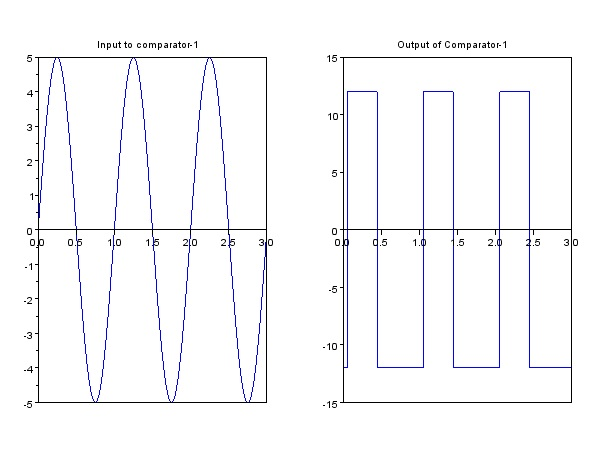
\includegraphics[width=6in]{../61/CH13/EX13.1/ex13_1.jpg}
\caption{Comparator}
\end{figure}

\vspace*{10mm}
\curlable{Exa~13.1}
\begin{code}
\tcaption{Comparator}{Comparator}
\lstinputlisting{../61/CH13/EX13.1/ex13_1.sce}
\end{code}

\vspace*{10mm}
\curlable{Exa~13.2}
\begin{code}
\tcaption{Trigger points}{Trigger points}
\lstinputlisting{../61/CH13/EX13.2/ex13_2.sce}
\end{code}

\vspace*{10mm}
\curlable{Fig~13.3}
\begin{figure}
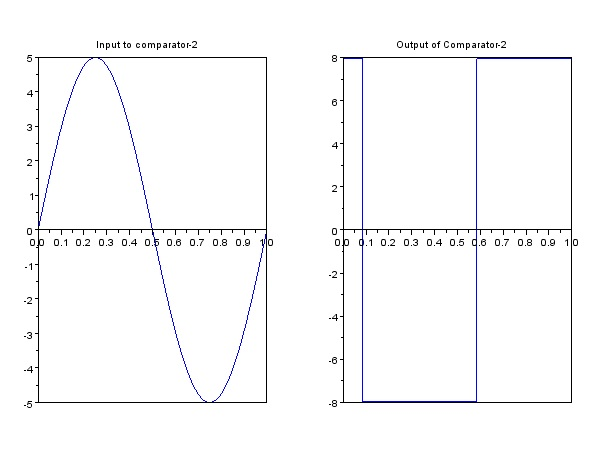
\includegraphics[width=6in]{../61/CH13/EX13.3/ex13_3.jpg}
\caption{Comparator hysteris Zener bounding}
\end{figure}

\vspace*{10mm}
\curlable{Exa~13.3}
\begin{code}
\tcaption{Comparator hysteris Zener bounding}{Comparator hysteris Zener bounding}
\lstinputlisting{../61/CH13/EX13.3/ex13_3.sce}
\end{code}

\vspace*{10mm}
\curlable{Exa~13.4}
\begin{code}
\tcaption{Summing amplifier unity gain}{Summing amplifier unity gain}
\lstinputlisting{../61/CH13/EX13.4/ex13_4.sce}
\end{code}

\vspace*{10mm}
\curlable{Exa~13.5}
\begin{code}
\tcaption{Summing amplifier}{Summing amplifier}
\lstinputlisting{../61/CH13/EX13.5/ex13_5.sce}
\end{code}

\vspace*{10mm}
\curlable{Exa~13.6}
\begin{code}
\tcaption{Averaging amplifier}{Averaging amplifier}
\lstinputlisting{../61/CH13/EX13.6/ex13_6.sce}
\end{code}

\vspace*{10mm}
\curlable{Exa~13.7}
\begin{code}
\tcaption{Scaling adder}{Scaling adder}
\lstinputlisting{../61/CH13/EX13.7/ex13_7.sce}
\end{code}

\vspace*{10mm}
\curlable{Fig~13.8}
\begin{figure}
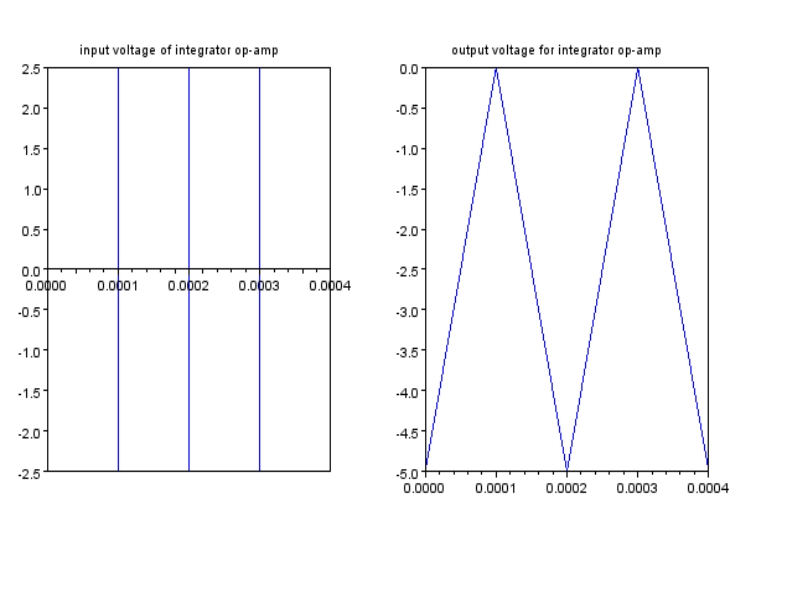
\includegraphics[width=6in]{../61/CH13/EX13.8/ex13_8.jpg}
\caption{Opamp integrator}
\end{figure}

\vspace*{10mm}
\curlable{Exa~13.8}
\begin{code}
\tcaption{Opamp integrator}{Opamp integrator}
\lstinputlisting{../61/CH13/EX13.8/ex13_8.sce}
\end{code}

\vspace*{10mm}
\curlable{Fig~13.9}
\begin{figure}
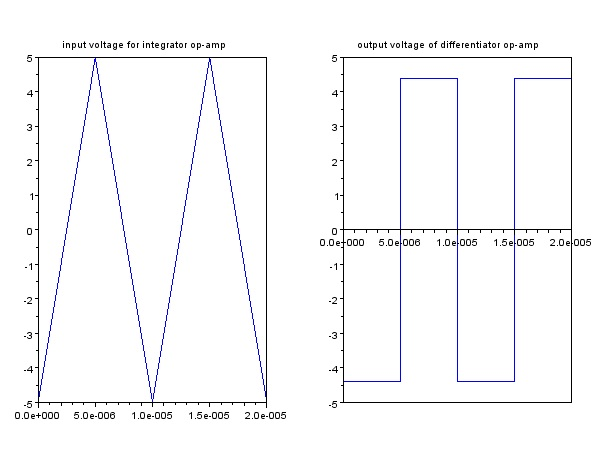
\includegraphics[width=6in]{../61/CH13/EX13.9/ex13_9.jpg}
\caption{Opamp differentiator}
\end{figure}

\vspace*{10mm}
\curlable{Exa~13.9}
\begin{code}
\tcaption{Opamp differentiator}{Opamp differentiator}
\lstinputlisting{../61/CH13/EX13.9/ex13_9.sce}
\end{code}

\chapter{Special Purpose Opamp Circuits}

\vspace*{10mm}
\curlable{Exa~14.1}
\begin{code}
\tcaption{Gain setting resistor}{Gain setting resistor}
\lstinputlisting{../61/CH14/EX14.1/ex14_1.sce}
\end{code}

\vspace*{10mm}
\curlable{Exa~14.2}
\begin{code}
\tcaption{Voltage gain Instrumentation amplifier}{Voltage gain Instrumentation amplifier}
\lstinputlisting{../61/CH14/EX14.2/ex14_2.sce}
\end{code}

\vspace*{10mm}
\curlable{Exa~14.3}
\begin{code}
\tcaption{Isolation amplifier}{Isolation amplifier}
\lstinputlisting{../61/CH14/EX14.3/ex14_3.sce}
\end{code}

\vspace*{10mm}
\curlable{Exa~14.4}
\begin{code}
\tcaption{Voltage gain Isolation amplifier}{Voltage gain Isolation amplifier}
\lstinputlisting{../61/CH14/EX14.4/ex14_4.sce}
\end{code}

\vspace*{10mm}
\curlable{Exa~14.5}
\begin{code}
\tcaption{Transconductance OTA}{Transconductance OTA}
\lstinputlisting{../61/CH14/EX14.5/ex14_5.sce}
\end{code}

\vspace*{10mm}
\curlable{Exa~14.6}
\begin{code}
\tcaption{Voltage gain OTA}{Voltage gain OTA}
\lstinputlisting{../61/CH14/EX14.6/ex14_6.sce}
\end{code}

\vspace*{10mm}
\curlable{Fig~14.7}
\begin{figure}
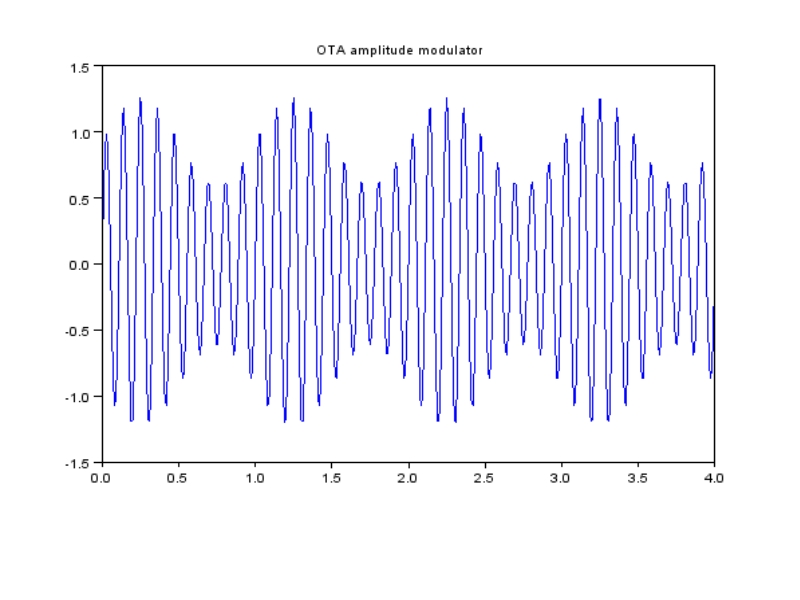
\includegraphics[width=6in]{../61/CH14/EX14.7/ex14_7.jpg}
\caption{Output OTA amplitude modulator}
\end{figure}

\vspace*{10mm}
\curlable{Exa~14.7}
\begin{code}
\tcaption{Output OTA amplitude modulator}{Output OTA amplitude modulator}
\lstinputlisting{../61/CH14/EX14.7/ex14_7.sce}
\end{code}

\vspace*{10mm}
\curlable{Exa~14.8}
\begin{code}
\tcaption{Output log amplifier}{Output log amplifier}
\lstinputlisting{../61/CH14/EX14.8/ex14_8.sce}
\end{code}

\vspace*{10mm}
\curlable{Exa~14.9}
\begin{code}
\tcaption{Transistor log amplifier}{Transistor log amplifier}
\lstinputlisting{../61/CH14/EX14.9/ex14_9.sce}
\end{code}

\vspace*{10mm}
\curlable{Exa~14.10}
\begin{code}
\tcaption{Antilog amplifier}{Antilog amplifier}
\lstinputlisting{../61/CH14/EX14.10/ex14_10.sce}
\end{code}

\chapter{Active Filters}

\vspace*{10mm}
\curlable{Exa~15.1}
\begin{code}
\tcaption{Band pass filter}{Band pass filter}
\lstinputlisting{../61/CH15/EX15.1/ex15_1.sce}
\end{code}

\vspace*{10mm}
\curlable{Exa~15.2}
\begin{code}
\tcaption{Butterworth response}{Butterworth response}
\lstinputlisting{../61/CH15/EX15.2/ex15_2.sce}
\end{code}

\vspace*{10mm}
\curlable{Exa~15.3}
\begin{code}
\tcaption{Sallen Key lowpass filter}{Sallen Key lowpass filter}
\lstinputlisting{../61/CH15/EX15.3/ex15_3.sce}
\end{code}

\vspace*{10mm}
\curlable{Exa~15.4}
\begin{code}
\tcaption{4 pole filter}{4 pole filter}
\lstinputlisting{../61/CH15/EX15.4/ex15_4.sce}
\end{code}

\vspace*{10mm}
\curlable{Exa~15.5}
\begin{code}
\tcaption{Sallen Key highpass filter}{Sallen Key highpass filter}
\lstinputlisting{../61/CH15/EX15.5/ex15_5.sce}
\end{code}

\vspace*{10mm}
\curlable{Exa~15.6}
\begin{code}
\tcaption{Cascaded filter}{Cascaded filter}
\lstinputlisting{../61/CH15/EX15.6/ex15_6.sce}
\end{code}

\vspace*{10mm}
\curlable{Exa~15.7}
\begin{code}
\tcaption{State variable filter}{State variable filter}
\lstinputlisting{../61/CH15/EX15.7/ex15_7.sce}
\end{code}

\vspace*{10mm}
\curlable{Exa~15.8}
\begin{code}
\tcaption{Band stop filter}{Band stop filter}
\lstinputlisting{../61/CH15/EX15.8/ex15_8.sce}
\end{code}

\chapter{Oscillators}

\vspace*{10mm}
\curlable{Exa~16.1}
\begin{code}
\tcaption{Wien bridge oscillator}{Wien bridge oscillator}
\lstinputlisting{../61/CH16/EX16.1/ex16_1.sce}
\end{code}

\vspace*{10mm}
\curlable{Exa~16.2}
\begin{code}
\tcaption{Phase shift oscillator}{Phase shift oscillator}
\lstinputlisting{../61/CH16/EX16.2/ex16_2.sce}
\end{code}

\vspace*{10mm}
\curlable{Exa~16.3}
\begin{code}
\tcaption{FET Colpitts oscillator}{FET Colpitts oscillator}
\lstinputlisting{../61/CH16/EX16.3/ex16_3.sce}
\end{code}

\vspace*{10mm}
\curlable{Exa~16.4}
\begin{code}
\tcaption{Triangular wave oscillator}{Triangular wave oscillator}
\lstinputlisting{../61/CH16/EX16.4/ex16_4.sce}
\end{code}

\vspace*{10mm}
\curlable{Fig~16.5}
\begin{figure}
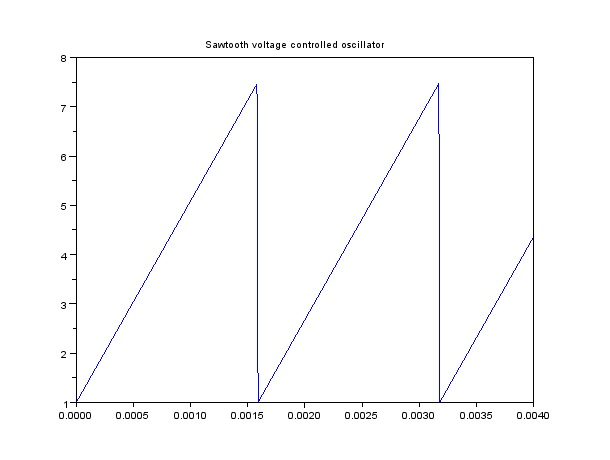
\includegraphics[width=6in]{../61/CH16/EX16.5/ex16_5.jpg}
\caption{Sawtooth VCO}
\end{figure}

\vspace*{10mm}
\curlable{Exa~16.5}
\begin{code}
\tcaption{Sawtooth VCO}{Sawtooth VCO}
\lstinputlisting{../61/CH16/EX16.5/ex16_5.sce}
\end{code}

\vspace*{10mm}
\curlable{Exa~16.6}
\begin{code}
\tcaption{555 timer}{555 timer}
\lstinputlisting{../61/CH16/EX16.6/ex16_6.sce}
\end{code}

\chapter{Voltage Regulators}

\vspace*{10mm}
\curlable{Exa~17.1}
\begin{code}
\tcaption{Percentage line regulation}{Percentage line regulation}
\lstinputlisting{../61/CH17/EX17.1/ex17_1.sce}
\end{code}

\vspace*{10mm}
\curlable{Exa~17.2}
\begin{code}
\tcaption{Load regulation percentage}{Load regulation percentage}
\lstinputlisting{../61/CH17/EX17.2/ex17_2.sce}
\end{code}

\vspace*{10mm}
\curlable{Exa~17.3}
\begin{code}
\tcaption{Series regulator}{Series regulator}
\lstinputlisting{../61/CH17/EX17.3/ex17_3.sce}
\end{code}

\vspace*{10mm}
\curlable{Exa~17.4}
\begin{code}
\tcaption{Overload protection}{Overload protection}
\lstinputlisting{../61/CH17/EX17.4/ex17_4.sce}
\end{code}

\vspace*{10mm}
\curlable{Exa~17.5}
\begin{code}
\tcaption{Shunt regulator}{Shunt regulator}
\lstinputlisting{../61/CH17/EX17.5/ex17_5.sce}
\end{code}

\vspace*{10mm}
\curlable{Exa~17.6}
\begin{code}
\tcaption{Positive linear voltage regulator}{Positive linear voltage regulator}
\lstinputlisting{../61/CH17/EX17.6/ex17_6.sce}
\end{code}

\vspace*{10mm}
\curlable{Exa~17.7}
\begin{code}
\tcaption{External pass filter}{External pass filter}
\lstinputlisting{../61/CH17/EX17.7/ex17_7.sce}
\end{code}

\vspace*{10mm}
\curlable{Exa~17.8}
\begin{code}
\tcaption{Power rating 7824}{Power rating 7824}
\lstinputlisting{../61/CH17/EX17.8/ex17_8.sce}
\end{code}

\vspace*{10mm}
\curlable{Exa~17.9}
\begin{code}
\tcaption{Current regulator}{Current regulator}
\lstinputlisting{../61/CH17/EX17.9/ex17_9.sce}
\end{code}

\chapter{Programmable Analog Arrays}

\vspace*{10mm}
\curlable{Exa~18.1}
\begin{code}
\tcaption{Switching capacitor}{Switching capacitor}
\lstinputlisting{../61/CH18/EX18.1/ex18_1.sce}
\end{code}

\chapter*{Appendix}
\curlable{AP~1}
\begin{code}
\label{AP:9}
\tcaption {Phase shift in degrees}{Phase shift in degrees}
\lstinputlisting{../61/DEPENDENCIES/phase_shift.sci}
\end{code}

\curlable{AP~2}
\begin{code}
\label{AP:8}
\tcaption {Open loop gain}{Open loop gain}
\lstinputlisting{../61/DEPENDENCIES/open_loop_gain.sci}
\end{code}

\curlable{AP~3}
\begin{code}
\label{AP:7}
\tcaption {Voltage gain in decibel}{Voltage gain in decibel}
\lstinputlisting{../61/DEPENDENCIES/gain_in_decibel_voltage.sci}
\end{code}

\curlable{AP~4}
\begin{code}
\label{AP:6}
\tcaption {Power gain in decibel}{Power gain in decibel}
\lstinputlisting{../61/DEPENDENCIES/gain_in_decibel_power.sci}
\end{code}

\curlable{AP~5}
\begin{code}
\label{AP:5}
\tcaption {value of K}{value of K}
\lstinputlisting{../61/DEPENDENCIES/value_of_K.sci}
\end{code}

\curlable{AP~6}
\begin{code}
\label{AP:4}
\tcaption {Drain current value}{Drain current value}
\lstinputlisting{../61/DEPENDENCIES/value_of_I_D.sci}
\end{code}

\end{document}
